\section{Electromagnetism Physics}
    \subsection{Capacitor}
        \paragraph{Property of capacitor}
            For parallel plate capacitor shown in Figure \ref{capa_struct}, the area of each plate is $A$, the distance between two plates is $d$, the permittivity of the filling is $\epsilon$.
            \begin{figure}[H]
                \begin{center}
                    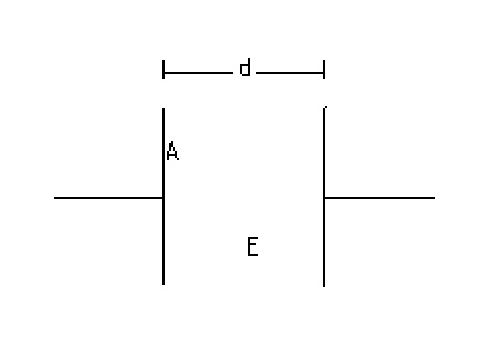
\includegraphics[height=3cm]{electromagnetism_charts/capa_struct.eps}
                \end{center}
                \caption{Structure of a capacitor}
                \label{capa_struct}
            \end{figure}

            Permittivity is relative permittivity $k$ times vacuum dielectric constant $\epsilon_0$.
            \begin{align}
                \epsilon &= k \epsilon_0 \\
                         &= 8.85 \times 10^{-12} k
            \end{align}

            The capacitance is
            \begin{align}
                C = \epsilon \frac{A}{d}
            \end{align}

            The relation of voltage between two plates $U$ and charge on plates $Q$ is
            \begin{align}
                Q = C U
            \end{align}

        \paragraph{Connection of capacitor}
            Parallel connection is shown in Figure \ref{capa_para_conn}
            \begin{figure}[H]
                \begin{center}
                    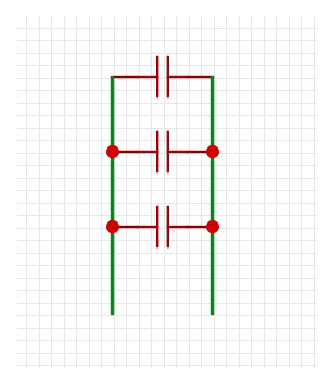
\includegraphics[height=3cm]{electromagnetism_charts/capa_para_conn.eps}
                \end{center}
                \caption{Capacitor parallel connection}
                \label{capa_para_conn}
            \end{figure}

            The resultant capacitance is
            \begin{align}
                C_T &= \frac{Q_T}{U_T} \\
                         &= \frac{\Sigma Q_i}{U_0} \\
                         &= \Sigma C_i
            \end{align}

            Serial connection is shown in Figure \ref{capa_seri_conn}

            \begin{figure}[H]
                \begin{center}
                    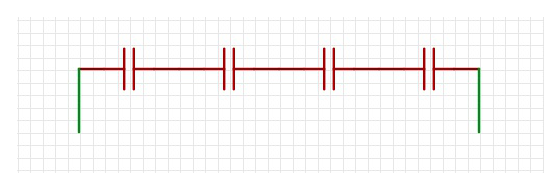
\includegraphics[height=2cm]{electromagnetism_charts/capa_seri_conn.eps}
                \end{center}
                \caption{Capacitor serial connection}
                \label{capa_seri_conn}
            \end{figure}

            The resultant capacitance is
            \begin{align}
                C_T &= \frac{Q_T}{U_T} = \frac{Q_0}{\Sigma U_i} \\
                \Rightarrow \frac{1}{C_T} &= \frac{\Sigma Ui}{Q_0} = \Sigma \frac{1}{C_i}
                % \Rightarrow C_T &= \frac{\Pi C_i}{\Sigma C_i}
            \end{align}

        \paragraph{Charging the capacitor}
            Figure \ref{charge_capa} shows charging a capacitor with capacitance $C$ through a resistance $R$ with voltage $\epsilon$.

            \begin{figure}[H]
                \begin{center}
                    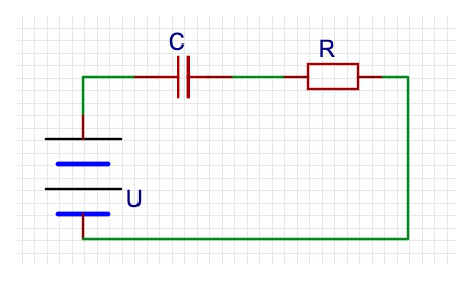
\includegraphics[height=3cm]{electromagnetism_charts/charge_capa.eps}
                \end{center}
                \caption{Charge capacitor}
                \label{charge_capa}
            \end{figure}

            \begin{align}
                Q(t) &= C U(t) \label{charge_capa_qtcu} \\ 
                \epsilon &= I(t) R + U(t) \label{charge_capa_euir}\\
                Q(t) &= \int_{0}^{t} I(t) \mathrm{d} t \label{charge_capa_qtit}
            \end{align}

            From Equation \ref{charge_capa_qtcu} and Equation \ref{charge_capa_qtit}, 
            \begin{align}
                & C U(t) = \int_{0}^{t} I(t) \mathrm{d} t \\
                & \therefore C \frac{\mathrm{d} U(t)}{\mathrm{d} t} = I(t)
            \end{align}

            From Equation \ref{charge_capa_euir},
            \begin{align}
                U(t) = \epsilon - I(t) R \\
                \therefore \frac{\mathrm{d} U(t)}{\mathrm{d} t} = -R \frac{\mathrm{d} I(t)}{\mathrm{d} t}
            \end{align}

            \begin{align}
                & \therefore \frac{I(t)}{C} = - R \frac{\mathrm{d} I(t)}{\mathrm{d} t} \\
                & \therefore \frac{\mathrm{d} I(t)}{I(t)} = \frac{\mathrm{d} t}{- C R} \\
                & \therefore I(t) = A e^{- \frac{t}{RC}}
            \end{align}

            \begin{align}
                & \because \mbox{when\ } t = 0, I(t) = \frac{\epsilon}{R} \\
                & \therefore A = \frac{\epsilon}{R} \\
                & \therefore I(t) = \frac{\epsilon}{R} e^{- \frac{t}{RC}}
            \end{align}

            \begin{align}
                \therefore & U(t) = \epsilon - I(t) R = \epsilon (1 - e^{- \frac{t}{RC}}) \\
                           & Q(t) = C U(t) = \epsilon C (1 - e^{- \frac{t}{RC}})
            \end{align}

        \paragraph{Discharging the capacitor}
            Figure \ref{discha_capa} shows discharging a capacitor with capacitance $C$ and initial voltage $U_0$ across a resistance $R$. 

            \begin{figure}[H]
                \begin{center}
                    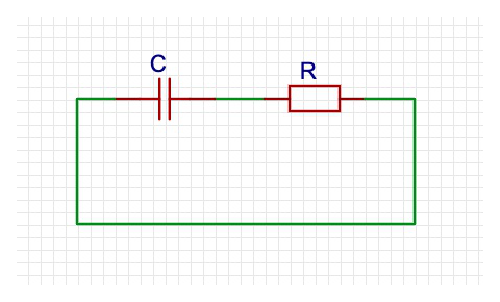
\includegraphics[height=3cm]{electromagnetism_charts/discha_capa.eps}
                \end{center}
                \caption{Discharge capacitor}
                \label{discha_capa}
            \end{figure}

            \begin{align}
                Q(t) &= C U(t) \label{discha_qtcu} \\
                U(t) &= I(t) R \label{discha_utir} \\
                Q(t) &= C U_0 - \int_{0}^{t} I(t) \mathrm{d} t \label{discha_qtit}
            \end{align}

            From Equation \ref{discha_qtcu} and Equation \ref{discha_qtit},
            \begin{align}
                CU(t) = CU_0 - \int I(t) \mathrm{d} t \label{discha_fm1_3}
            \end{align}

            Substitude Equation \ref{discha_utir} into Equation \ref{discha_fm1_3}, 
            \begin{align}
                & C R I(t) = C U_0 - \int  I(t) \mathrm{d} t \\
                & \therefore C R \frac{\mathrm{d} I(t)}{\mathrm{d} t} = - I(t) \\
                & \therefore - C R \int \frac{1}{I(t)} \mathrm{d} t = \int \mathrm{d} t \\
                & \therefore I(t) = A e^{- \frac{t}{RC}}
            \end{align}

            \begin{align}
                & \because \mbox{when\ } t = 0, I(t) = \frac{U_0}{R} \\
                & \therefore I(t) = \frac{U_0}{R} e^{- \frac{t}{RC}}
            \end{align}

            \begin{align}
                \therefore  U(t) &= I(t) R = U_0 e^{- \frac{t}{RC}} \\
                            Q(t) &= C U(t) = C U_0 e^{- \frac{t}{RC}} \\
                                 &= Q_0 e^{- \frac{t}{RC}}
            \end{align}

        \paragraph{Time constant}
            Time constant, $\tau$, defined as $\tau = RC$. 

            Define $t_{1/2}$ be the time to charge the capacitor to a half full. $\tau = \frac{t_{1/2}}{\ln 2}$. Proof:

            \begin{align}
                & U(t_{1/2}) = \epsilon (1 - e^{- \frac{t_{1/2}}{\tau}}) = \frac{1}{2} \epsilon \\
                & \Rightarrow e^{- \frac{t_{1/2}}{\tau}} = 2^{-1} \\
                & \Rightarrow -\frac{t_{1/2}}{\tau} = \ln (2^{-1}) \\
                & \Rightarrow \frac{t_{1/2}}{\tau} = \ln 2 \\
                & \Rightarrow \tau = \frac{t_{1/2}}{\ln 2}
            \end{align}

        % TODO: When insert dioele, where energy go?

    \subsection{Lorentz's force}
        Moving charge in a magnetic field is exerted with a Lorentz force. Is
        \begin{align}
            \vec{F} = q \vec{v} \vec{B}
        \end{align}

        Since force vector is always perpendicular to speed vector, the charge will circular motion in uniform magnetic field.

        In Figure \ref{llz_force}, an tiny object with mass $m$ and charge $q$ shoot into a uniform magnetic field with speed $v$. 
        \begin{figure}[H]
            \begin{center}
                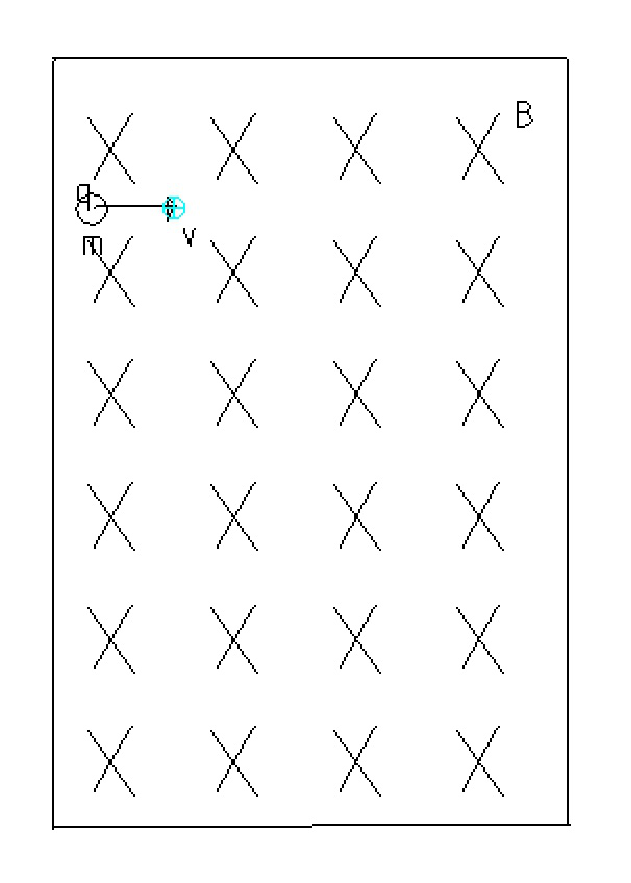
\includegraphics[height=5cm]{electromagnetism_charts/llz_force.eps}
            \end{center}
            \caption{Charge exerted with Lorentz force}
            \label{llz_force}
        \end{figure}

        The radius of circular motion is
        \begin{align}
            F &= q v B = m \frac{v^2}{r} \\
            \Rightarrow r &= \frac{m v}{B q}
        \end{align}

    \subsection{Ampere's force}
        Current in magnetic field exerted with Ampere's force. 
        \begin{align}
            F &= Q \vec{v} \vec{B} \\
              &= I t \vec{v} \vec{B} \\
              &= I \vec{L} \vec{B}
        \end{align}

        

    \subsection{Electronic Magnetic Induction}
        
        \paragraph{Conductor cut magnetic field line}
            In Figure \ref{cut_fieldline} is a conductor moving perpendicular to field line with speed $v$ in magnetic field with strength $B$.

            \begin{figure}[H]
                \begin{center}
                    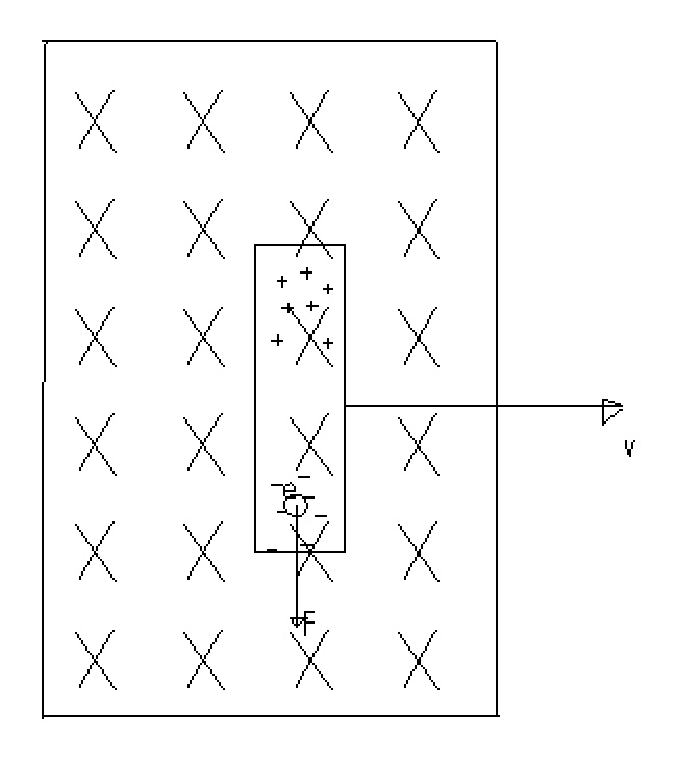
\includegraphics[height=4cm]{electromagnetism_charts/cut_fieldline.eps}
                \end{center}
                \caption{Conductor cut magnetic field line}
                \label{cut_fieldline}
            \end{figure}

            The electrons in the conductor suffer Lorentz force and move down. As a resultant, upper end get positive charge and bottom end get negative charge.

            The potential difference induced is called motional emf.
        
        \paragraph{Magnetic flux}
            $\phi$, defined by Faraday in 1831, 
            \begin{align}
                \phi = B \cdot A \cdot \cos(\theta)
            \end{align}
            Here $\theta$ is the angle between the normal to the area and the magnetic field.

            The unit is $\mathrm{Tm^2}$ or $\mathrm{Wb}$.

            If there is $N$ loops, 
            \begin{align}
                \phi = N B A \cos\theta
            \end{align}

        \paragraph{Faraday law}
            \begin{align}
                \epsilon \propto \frac{\mathrm{d} \phi}{\mathrm{d} t}
            \end{align}

            For coil with $N$ circles, the emf is
            \begin{align}
                \epsilon = -N \frac{\mathrm{d} \phi}{\mathrm{d} t}
            \end{align}

            % TODO: 楞次定律, 滑杆, 受力方向
        
        \paragraph{Slide-conductor model}
            In Figure \ref{sli_con_mod}, the length of conductor is $l$, sliding speed is $v$, magnetic field strength is $B$.
            \begin{figure}[H]
                \begin{center}
                    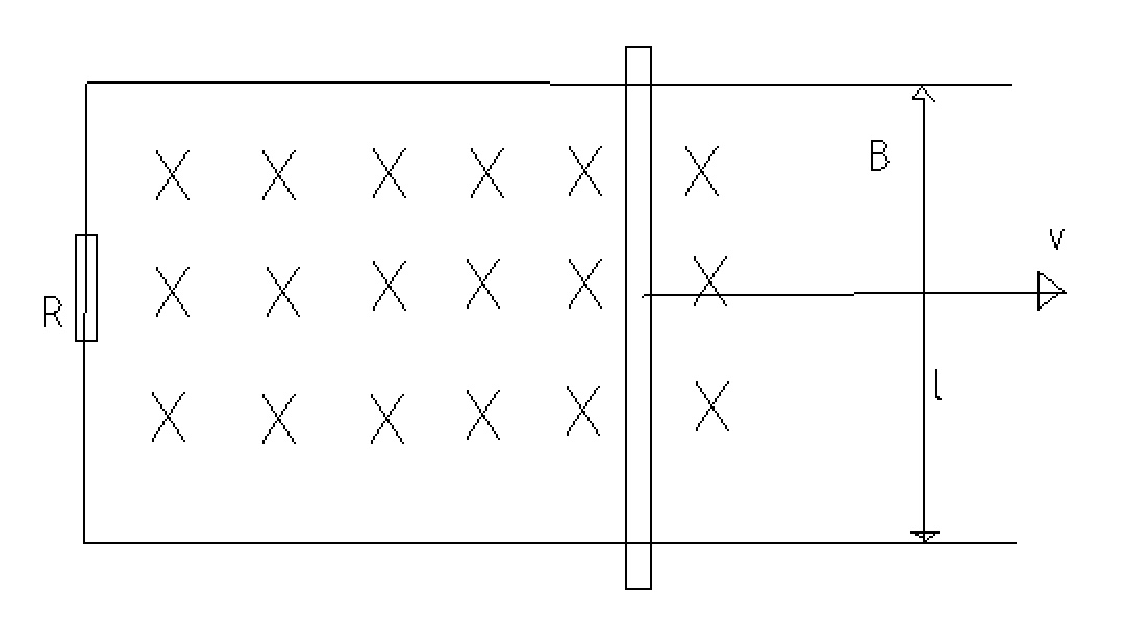
\includegraphics[height=4cm]{electromagnetism_charts/slide_cond.eps}
                \end{center}
                \caption{Slide conductor model}
                \label{sli_con_mod}
            \end{figure}

            The motional emf is
            \begin{align}
                \epsilon &= N \frac{\mathrm{d} \phi}{\mathrm{d} t} \\
                         &= N B \frac{\mathrm{d} A}{\mathrm{d} t} \\
                         &= N B l v \\
                         &= B l v
            \end{align}

            The current in loop is
            \begin{align}
                I &= \frac{\epsilon}{R}
            \end{align}

            The induced resistance force is
            \begin{align}
                F &= B I L \\
                  &= B \frac{\epsilon}{R} l \\
                  &= B \frac{B l v}{R} l \\
                  &= \frac{B^2 l^2 v}{R}
            \end{align}

            Direction is opposite to direction of sliding. (Energy conservation)

    \subsection{Power transformation}
        \paragraph{Power generator}
            Figure \ref{generator} shows a generator model.

            \begin{figure}[H]
                \begin{center}
                    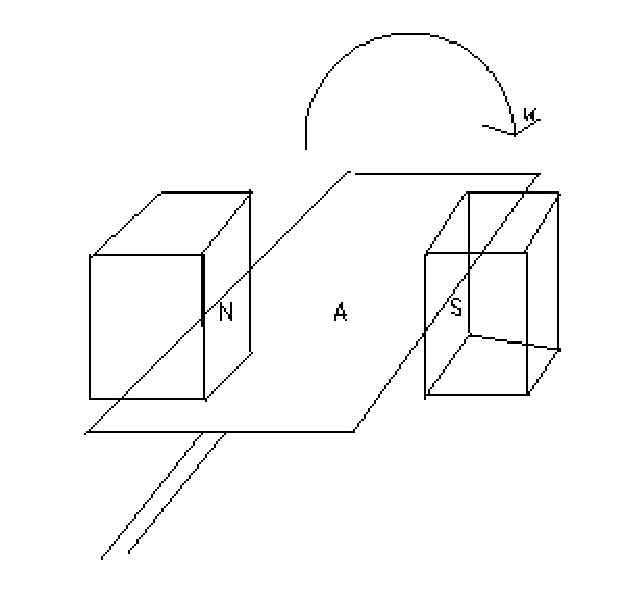
\includegraphics[height=5cm]{electromagnetism_charts/generator.eps}
                \end{center}
                \caption{Generator}
                \label{generator}
            \end{figure}

            The rotor is rotate at angular speed $\omega$. The cross-area of rotor is $A_0$. There are $N$ loops in the rotor. The output voltage is

            \begin{align}
                \epsilon &= N B \frac{\mathrm{d} A}{\mathrm{d} t} \\
                         &= N B \frac{\mathrm{d} (\sin (\omega t) A_0)}{\mathrm{d} t} \\
                         &= N B \omega A_0 \cos (\omega t) \\
                         & \mbox{Equivalent to} \\
                         & \ \ \ N B \omega A_0 \sin (\omega t)
            \end{align}

            The power is
            \begin{align}
                P &= \frac{{\epsilon_{\mathrm{rms}}}^2}{R}\\
                  &= \frac{(N B \omega A)^2}{2 R}
            \end{align}

        \paragraph{Alternating Current}
            A.C., the relation of voltage to time is sine function. 
            \begin{align}
                U = U_0 \sin (2 \pi f t)
            \end{align}

            The root-mean-square voltage, $\sqrt{\bar{u^2}}$, is
            \begin{align}
                U_{\mathrm{rms}} = \frac{U_0}{\sqrt{2}}
            \end{align}

            Power:
            \begin{align}
                P &= \frac{{U_{\mathrm{rms}}}^2}{R} \\
                  &= \frac{{U_0}^2}{2 R}
            \end{align}

        \paragraph{Voltage transformer}
            Figure \ref{transformer} show a transformer. The input coil have $N_1$ loops, input voltage is $U_1$, output coil have $N_2$ loops, output voltage is $U_2$.

            \begin{figure}[H]
                \begin{center}
                    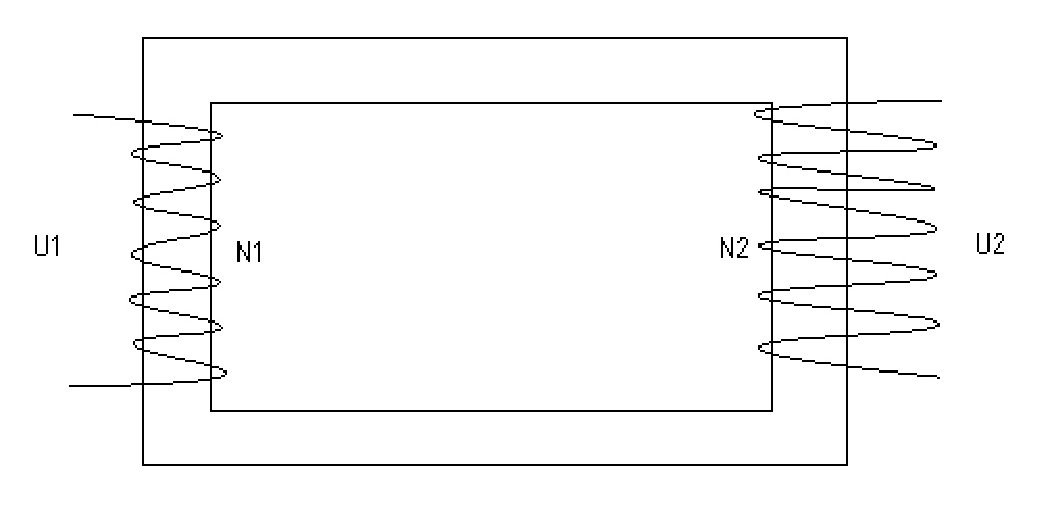
\includegraphics[height=4cm]{electromagnetism_charts/transformer.eps}
                \end{center}
                \caption{Transformer}
                \label{transformer}
            \end{figure}

            \begin{align}
                \frac{U_1}{N_1} = \frac{U_2}{N_2}
            \end{align}
            
            Eddy current: current in iron that may leed to energy loss.

            Ways to avoid energy loss:
            \begin{enumerate}
                \item Slice the iron into pieces and use insulator to seperate them.
                \item Use higher voltage.
            \end{enumerate}